\begin{frame}[plain]
    \begin{center}
        \vspace{48pt}
        {\huge\bf センサーを使った応用}
    \end{center}
\end{frame}

\begin{frame}
    \frametitle{センサーをピンにつけてみよう}
    \begin{center}
        \begin{columns}
            \begin{column}{0.48\textwidth}
                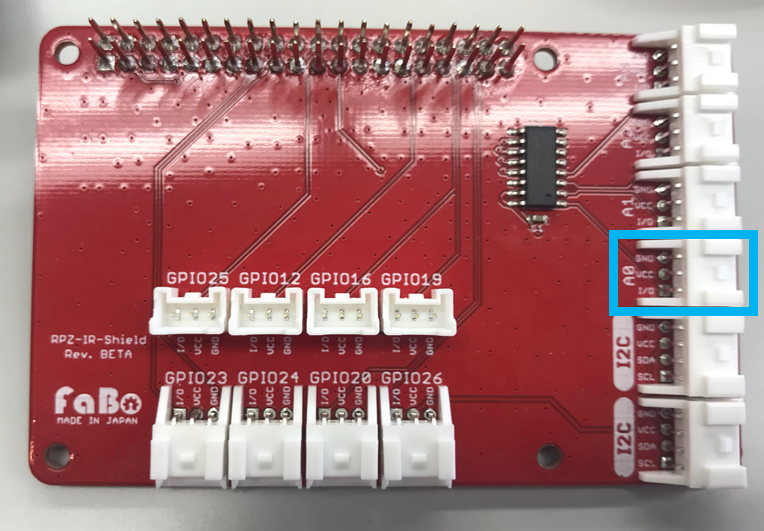
\includegraphics[width=0.8\textwidth]{images/chap05/text05-img030.png}
            \end{column}
            \begin{column}{0.48\textwidth}
                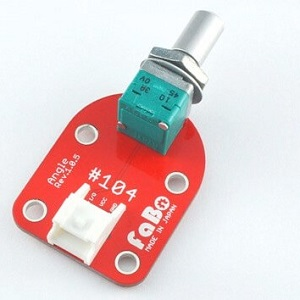
\includegraphics[width=0.8\textwidth]{images/chap05/text05-img022.jpg} 
            \end{column}
        \end{columns}
        \begin{itemize}
            \item A0とボリュームをつなげてみよう
            \item HSPでangle.hspを動かしてみよう
        \end{itemize}
    \end{center}
\end{frame}

\begin{frame}[fragile]
    \frametitle{ボリュームを使って画像を動かそう(angle.hsp)}
\begin{lstlisting}
#include "hsp3dish.as"
#include "rpz-gpio.as"

celload("hyou.png"),2
p = 50

spiopen 0

*main
	data = spiget(0,0)
	p = rasp_map(data, 0, 1023, 0, 440)

	redraw 0
	pos 100,100
	mes data
	mes p
	pos 0,0
	celput 2
	redraw 1

	wait 10	
	goto *main

spiclose 0
\end{lstlisting}
\end{frame}

\begin{frame}[fragile]
    \frametitle{入力の値の範囲(はんい)を変える関数}
    {rasp\_map(値,入力された値の最小サイズ,入力された値の最大サイズ,出力する値の最小サイズ,出力する値の最大サイズ)}
\end{frame}

\begin{frame}[fragile]
    \frametitle{画像の場所}
    {画面のサイズは横が640、たてが480\\
    今回の画像のサイズは横が200、たてが150\\
    なので一番右に画像を置きたいときは \\
    画面のサイズ-画像のサイズを考えよう}
\end{frame}

\begin{frame}[fragile]
    \frametitle{問題を解いてみよう}
    \begin{itemize}
        \item 教科書23ページ 問題5-10
        \begin{itemize}
            \item 6問は授業中にやる
        \end{itemize}
        \item 教科書24ページ 問題5-11
        \begin{itemize}
            \item 2問は宿題。時間があれば授業中にやる
        \end{itemize}
    \end{itemize}
\end{frame}

\begin{frame}[fragile]
    \frametitle{LEDの明るさを変えよう(pwm.hsp)}
\begin{lstlisting}
#include "hsp3dish.as"
#include "rpz-gpio.as"

redraw 0
redraw 1

repeat
gpio 27,1

repeat 200
if cnt < 10 : gpio 17,1 : else : gpio 17,0
if cnt < 50 : gpio 18,1 : else : gpio 18,0
if cnt < 100 : gpio 22,1 : else : gpio 22,0
loop

await 1
loop

gpio 17,0
gpio 18,0
gpio 22,0
gpio 27,0
stop
\end{lstlisting}
\end{frame}

\begin{frame}
    \frametitle{LEDの明るさに強弱をつけるには}
    \begin{center}
        \begin{figure}
            \includesvg[width=0.8\linewidth]{images/chap05/led_frequency.svg}
        \end{figure}
        \begin{itemize}
            \item 一定時間のLEDの消灯時間の比率で明るさに強弱をつけることができる
        \end{itemize}
    \end{center}
\end{frame}